\documentclass[14pt, aspectratio=169, xcolor={dvipsnames}]{beamer}

\hbadness=99999
\usepackage{silence}

\usepackage[T1]{fontenc}
\usepackage{fontawesome5}

\usepackage{soul}
\usepackage{csquotes}
\usepackage{textcomp}
\usepackage{listings}

\usepackage{amsmath}
\usepackage{amssymb}
\usepackage{amsfonts}
\usepackage{mathtools}
\usepackage{mathpartir}
\usepackage{bm}
\usepackage{relsize}
\usepackage{centernot}
\usepackage{stmaryrd}
\WarningFilter{latexfont}{Font shape `U/stmry/b/n' undefined}
\WarningFilter{latexfont}{Some font shapes were not available}

\usepackage{scalerel}
\usepackage[most]{tcolorbox}
\usepackage{framed}

\usepackage{pgfpages}
\usepackage{fancyvrb}
\usepackage{pgfplots}
\pgfplotsset{compat=1.18}

\usepackage[style=authoryear, sortcites, backend=biber]{biblatex}

\usepackage{tikz}
\usetikzlibrary{arrows, arrows.meta, shapes, calc, positioning, backgrounds, hobby}

% \ifnotes
\setbeamertemplate{note page}[plain]
\setbeameroption{show notes on second screen}
% \fi

\usetheme{auriga}
\usecolortheme{auriga}
% \setbeamercovered{transparent}

\makeatletter
\let\HL\hl
\renewcommand\hl{%
  \let\set@color\beamerorig@set@color
  \let\reset@color\beamerorig@reset@color
  \HL}
\makeatother

\makeatletter
\let\UL\ul
\renewcommand\ul{%
  \let\set@color\beamerorig@set@color
  \let\reset@color\beamerorig@reset@color
  \UL}
\makeatother

\newcommand{\undercolor}[2][Red]{\setulcolor{#1}\ul{#2}}
\newcommand<>{\onderline}[1]{\alt#2{\underline{#1}}{#1}}
\newcommand<>{\onderset}[2]{\alt#3{\underset{#1}{#2}}{#2}}

\tikzset{
  invisible/.style={opacity=0,text opacity=0},
  visible on/.style={alt={#1{}{invisible}}},
  alt/.code args={<#1>#2#3}{%
    \alt<#1>{\pgfkeysalso{#2}}{\pgfkeysalso{#3}}
  },
  Alt/.code args={<#1>#2#3}{%
    \Alt<#1>{\pgfkeysalso{#2}}{\pgfkeysalso{#3}}
  },
}

\pdfstringdefDisableCommands{%
  \def\\{}%
  \def\underline#1{<#1>}%
}

\colorlet{highlight}{yellow!30}

\tcbuselibrary{skins}
\tcbuselibrary{listings}
\tcbset{
  base/.style={
    arc=0mm, 
    bottomtitle=0.5mm,
    boxrule=0mm,
    colbacktitle=black!10!white, 
    coltitle=black!80!white, 
    fonttitle=\bfseries, 
    left=2.5mm,
    right=3.5mm,
    title={#1},
    toptitle=0.75mm, 
  }
}

\newtcolorbox{mainbox}[2][]{
  enhanced,
  colframe=black!30!white, 
  base={#2},
  #1
}

\newtcolorbox{subbox}[2][]{
  enhanced,
  colframe=black!20!white,
  base={#2},
  #1,
}

\lstloadlanguages{caml}
\lstdefinestyle{OCaml}{%
  language = caml,
  literate={"}{\textquotedbl}1,
  morekeywords = {assert, failwith},
}
\lstset{upquote=true}

\makeatletter
\def\beamer@checkframetitle{%
\begingroup
  \edef\temp{%
    \endgroup
    \noexpand\frametitle
    [\unexpanded\expandafter{\beamer@savedshortframetitle}]%
    {\unexpanded\expandafter{\beamer@savedframetitle}}%
  }
\temp
\@ifnextchar\bgroup\beamer@inlineframetitle{}}

\long\def\beamer@@frametitle[#1]#2{%
  \beamer@ifempty{#2}{}{%
    \gdef\insertframetitle{{#2\ifnum\beamer@autobreakcount>0\relax{}\space\usebeamertemplate*{frametitle
continuation}\fi}}%
  \gdef\beamer@frametitle{#2}%
  \gdef\beamer@shortframetitle{#1}%
  \global\let\beamer@savedshortframetitle\beamer@shortframetitle
    \global\let\beamer@savedframetitle\beamer@frametitle
}%
}
  \global\let\beamer@savedshortframetitle\@empty
    \global\let\beamer@savedframetitle\@empty

\makeatother

\makeatletter
\newcommand*\Alt{\alt{\Alt@branch0}{\Alt@branch1}}

\newcommand\Alt@branch[3]{%
  \begingroup
  \ifbool{mmode}{%
    \mathchoice{%
      \Alt@math#1{\displaystyle}{#2}{#3}%
    }{%
      \Alt@math#1{\textstyle}{#2}{#3}%
    }{%
      \Alt@math#1{\scriptstyle}{#2}{#3}%
    }{%
      \Alt@math#1{\scriptscriptstyle}{#2}{#3}%
    }%
  }{%
    \sbox0{#2}%
    \sbox1{#3}%
    \Alt@typeset#1%
  }%
  \endgroup
}

\newcommand\Alt@math[4]{%
  \sbox0{$#2{#3}\m@th$}%
  \sbox1{$#2{#4}\m@th$}%
  \Alt@typeset#1%
}

\newcommand\Alt@typeset[1]{%
  \ifnumcomp{\wd0}{>}{\wd1}{%
    \def\setwider   ##1##2{##2##1##2 0}%
    \def\setnarrower##1##2{##2##1##2 1}%
  }{%
    \def\setwider   ##1##2{##2##1##2 1}%
    \def\setnarrower##1##2{##2##1##2 0}%
  }%
  \sbox2{}%
  \sbox3{}%
  \setwider2{\wd}%
  \setwider2{\ht}%
  \setwider2{\dp}%
  \setnarrower3{\ht}%
  \setnarrower3{\dp}%
  \leavevmode
  \rlap{\usebox#1}%
  \usebox2%
  \usebox3%
}
\makeatother

\newcommand\wider[2][3em]{%
\makebox[\linewidth][c]{%
  \begin{minipage}{\dimexpr\textwidth+#1\relax}
  \raggedright#2
  \end{minipage}%
  }%
}

\makeatletter
\define@key {mprset}{style}[1]{\def\TirNameStyle{#1}}
\makeatother

\newenvironment{emphbox}[1]
  {\begin{leftbar}\vspace{0.3em}\textbf{#1}\\[0.5em]}
  {\vspace{0.3em}\end{leftbar}}

\newcommand{\ie}{\textit{i.e.}}
\newcommand{\eg}{\textit{e.g.}}
\newcommand{\wrt}{\textit{w.r.t.}}

\newcommand{\mousePointer}{\textcolor{Black!60}{\small\faMousePointer}}

%
% color
%
\newtcolorbox{highlightbox}[2][]{
  on line,
  hbox,
  boxsep=0pt,
  left=1pt,
  right=1pt,
  top=1pt,
  bottom=1pt,
  colframe=white,
  colback=#2
  #1,
}

\newcommand\goodcolor[2]{%
  \protect\leavevmode
  \begingroup
    \color{#1}%
    #2%
  \endgroup
}

\newcommand{\mathcolorbox}[2]{{\fboxsep=1pt\colorbox{#1}{$\displaystyle #2$}}}

%
% judgments
%
\newcommand{\judgbox}[1]{\noindent \fbox{$#1$}}

%
% math
%
\DeclareMathOperator{\?}{?}
\DeclareMathOperator{\dom}{dom}
\DeclareMathOperator{\cod}{cod}

\newcommand{\colorOkSideJudge}{Black!50}
\newcommand{\colorFailSideJudge}{red}

%
% relations
%

% equality
\newcommand{\equal}[2]{\ensuremath{#1 = #2}}
\newcommand{\notEqual}[2]{\ensuremath{\goodcolor{\colorFailSideJudge}{#1 \neq #2}}}

% consistency
\newcommand{\consistentRel}{\ensuremath{\sim}}
\newcommand{\consistent}[2]{\ensuremath{#1 \goodcolor{\colorOkSideJudge}{\consistentRel} #2}}
\newcommand{\inconsistentRel}{\ensuremath{\nsim}}
\newcommand{\inconsistent}[2]{\ensuremath{\goodcolor{\colorFailSideJudge}{#1 \inconsistentRel #2}}}

% matching
\newcommand{\matchedRel}[1]{\ensuremath{\blacktriangleright_{#1}}}
\newcommand{\notMatchedRel}[1]{\ensuremath{\blacktriangleright_{\centernot#1}}}
\newcommand{\matchedArrowRel}{\ensuremath{\matchedRel{\to}}}
\newcommand{\notMatchedArrowRel}{\ensuremath{\notMatchedRel{\to}}}
\newcommand{\matchedArrow}[3]{\ensuremath{#1 \goodcolor{\colorOkSideJudge}{\matchedArrowRel} \TArrow{#2}{#3}}}
\newcommand{\notMatchedArrow}[1]{\ensuremath{\goodcolor{\colorFailSideJudge}{#1 \notMatchedArrowRel}}}
\newcommand{\matchedProdRel}{\ensuremath{\matchedRel{\times}}}
\newcommand{\notMatchedProdRel}{\ensuremath{\notMatchedRel{\times}}}
\newcommand{\matchedProd}[3]{\ensuremath{#1 \goodcolor{\colorOkSideJudge}{\matchedProdRel} \TProd{#2}{#3}}}
\newcommand{\notMatchedProd}[1]{\ensuremath{\goodcolor{\colorFailSideJudge}{#1 \notMatchedProdRel}}}

% base types
\newcommand{\base}[1]{\ensuremath{#1 ~{\normalfont\textsf{base}}}}

% 
% syntax
%
\newcommand{\TMName}{{\normalfont\textsf{Type}}}
\newcommand{\TMSet}{\ensuremath{T}}
\newcommand{\TMV}{\ensuremath{\tau}}

\newcommand{\meetRel}{\sqcap}
\newcommand{\noMeetRel}{\centernot\sqcap}
\newcommand{\TMeet}[2]{\ensuremath{#1 \meetRel #2}}

\newcommand{\TUnknown}{\ensuremath{\?}}
\newcommand{\TUnknownSwitch}{\ensuremath{\?^{\Rightarrow}}}
\newcommand{\TNum}{\ensuremath{{\normalfont\textsf{num}}}}
\newcommand{\TBool}{\ensuremath{{\normalfont\textsf{bool}}}}
\newcommand{\TArrow}[2]{\ensuremath{#1 \goodcolor{\colorOkSideJudge}{\to} #2}}
\newcommand{\TProd}[2]{\ensuremath{#1 \times #2}}

%
% contexts
%
\newcommand{\ctx}{\ensuremath{\Gamma}}
\newcommand{\extendCtx}[3]{\ensuremath{#1 , ~\assignType{#2}{#3}}}
\newcommand{\inCtx}[3]{\ensuremath{\assignType{#2}{#3} \goodcolor{\colorOkSideJudge}{\in} #1}}
\newcommand{\notInCtx}[2]{\ensuremath{\goodcolor{\colorFailSideJudge}{#2 \not\in \dom(#1)}}}
\newcommand{\withCtx}[2]{\ensuremath{#1 \vdash #2}}

%
% typing
%
\newcommand{\assignType}[2]{\ensuremath{#1 \goodcolor{\colorOkSideJudge}{:} #2}}
\newcommand{\synType}[2]{\ensuremath{#1 \Rightarrow #2}}
\newcommand{\notSynType}[2]{\ensuremath{#1 \not\Rightarrow #2}}
\newcommand{\ctxSynType}[3]{\ensuremath{\withCtx{#1}{\synType{#2}{#3}}}}
\newcommand{\ctxNotSynType}[3]{\ensuremath{\withCtx{#1}{\notSynType{#2}{#3}}}}
\newcommand{\anaType}[2]{\ensuremath{#1 \Leftarrow #2}}
\newcommand{\notAnaType}[2]{\ensuremath{#1 \goodcolor{\colorFailSideJudge}{\not\Leftarrow} #2}}
\newcommand{\ctxAnaType}[3]{\ensuremath{\withCtx{#1}{\anaType{#2}{#3}}}}
\newcommand{\ctxNotAnaType}[3]{\ensuremath{\withCtx{#1}{\notAnaType{#2}{#3}}}}

% !requires types

%
% external expressions
%
\newcommand{\EMName}{{\normalfont\textsf{UExp}}}
\newcommand{\EMSet}{\ensuremath{E}}
\newcommand{\EMV}{\ensuremath{e}}

% holes
\newcommand{\EEHole}{\ensuremath{\ECEHole}}

% integers
\newcommand{\ENum}[1]{\ensuremath{\ECNum{#1}}}
\newcommand{\ENumMV}{\ensuremath{\ECNumMV}}
\newcommand{\EOpPlus}{\ensuremath{\ECOpPlus}}
\newcommand{\EPlus}[2]{\ensuremath{\ECPlus{#1}{#2}}}

% booleans
\newcommand{\ETrue}{\ensuremath{\ECTrue}}
\newcommand{\EFalse}{\ensuremath{\ECFalse}}
\newcommand{\EIf}[3]{\ensuremath{\ECIf{#1}{#2}{#3}}}
\newcommand{\EOpAnd}{\ensuremath{\ECOpAnd}}
\newcommand{\EAnd}[2]{\ensuremath{\ECAnd{#1}{#2}}}

% lambdas
\newcommand{\ELam}[3]{\ensuremath{\ECLam{#1}{#2}{#3}}}
\newcommand{\EAp}[2]{\ensuremath{\ECAp{#1}{#2}}}

% pairs
\newcommand{\EPair}[2]{\ensuremath{\ECPair{#1}{#2}}}
\newcommand{\EProjL}[1]{\ensuremath{\ECProjL{#1}}}
\newcommand{\EProjR}[1]{\ensuremath{\ECProjR{#1}}}

% let
\newcommand{\ELet}[3]{\ensuremath{\ECLet{#1}{#2}{#3}}}

%
% marked expressions
%
\newcommand{\ECMName}{{\normalfont\textsf{MExp}}}
\newcommand{\ECMSet}{\ensuremath{\check{E}}}
\newcommand{\ECMV}{\ensuremath{\check{e}}}

% holes
\definecolor{hole}{RGB}{162,85,162}
\newcommand{\ECEHole}{\ensuremath{\textcolor{hole}{\bm{\llparenthesis}}\textcolor{hole}{\bm{\rrparenthesis}}}}

\newcommand{\colorKeyword}{black!70}

% integers
\newcommand{\ECNum}[1]{\ensuremath{\goodcolor{Blue}{#1}}}
\newcommand{\ECNumMV}{\ensuremath{\ECNum{n}}}
\newcommand{\ECOpPlus}{\ensuremath{\goodcolor{\colorKeyword}{+}}}
\newcommand{\ECPlus}[2]{\ensuremath{#1 \ECOpPlus #2}}

% booleans
\newcommand{\ECTrue}{\ensuremath{{\normalfont\textsf{\textcolor{Purple}{true}}}}}
\newcommand{\ECFalse}{\ensuremath{{\normalfont\textsf{\textcolor{Purple}{false}}}}}
\newcommand{\ECIf}[3]{\ensuremath{\textsf{if}~ #1 ~\textsf{then}~ #2 ~\textsf{else}~ #3}}
\newcommand{\ECOpAnd}{\ensuremath{\mathbin{\goodcolor{\colorKeyword}{\text{\&\&}}}}}
\newcommand{\ECAnd}[2]{\ensuremath{#1 \ECOpAnd #2}}

% lambdas
\newcommand{\ECLam}[3]{\ensuremath{\goodcolor{\colorKeyword}{\lambda} #1 \goodcolor{\colorKeyword}{:} #2\goodcolor{\colorKeyword}{.} ~#3}}
\newcommand{\ECAp}[2]{\ensuremath{#1 ~#2}}

% pairs
\newcommand{\ECPair}[2]{\ensuremath{(#1, #2)}}
\newcommand{\ECProjL}[1]{\ensuremath{\pi_1 #1}}
\newcommand{\ECProjR}[1]{\ensuremath{\pi_2 #1}}

% let
\newcommand{\ECLet}[3]{\ensuremath{\textsf{let}~ #1 = #2 ~\textsf{in}~ #3}}

% errors
\newcommand{\MRFree}{\ensuremath{\mathsmaller{\mathsmaller{\mathsmaller{\square}}}}}
\newcommand{\MRInconType}{\ensuremath{\mathsmaller{\inconsistentRel}}}
\newcommand{\MRInconBr}{\ensuremath{{\noMeetRel}}}
\newcommand{\MRInconAsc}{\ensuremath{\bm{:}}}
\newcommand{\MRSynNonMatchedArrow}{\ensuremath{\mathsmaller{\notMatchedArrowRel}}}
\newcommand{\MRSynNonMatchedProd}{\ensuremath{\mathsmaller{\notMatchedProdRel}}}
\newcommand{\MRAnaNonMatchedArrow}{\ensuremath{\mathsmaller{\notMatchedArrowRel}}}
\newcommand{\MRAnaNonMatchedProd}{\ensuremath{\mathsmaller{\notMatchedProdRel}}}
\newcommand{\MRFreeTypeVar}{\ensuremath{\MRFree}}

\newcommand{\MRSyn}{\ensuremath{\mathsmaller{\Rightarrow}}}
\newcommand{\MRAna}{\ensuremath{\mathsmaller{\Leftarrow}}}

\newcommand{\ECMarked}[3]{\ensuremath{\goodcolor{red}{\bm{\llparenthesis}#1\bm{\rrparenthesis}_{#2}^{#3}}}}
\newcommand{\ECMarkedFree}[1]{\ensuremath{\ECMarked{#1}{\MRFree}{}}}
\newcommand{\ECMarkedInconType}[1]{\ensuremath{\ECMarked{#1}{\MRInconType}{}}}
\newcommand{\ECMarkedInconBr}[1]{\ensuremath{\ECMarked{#1}{\MRInconBr}{}}}
\newcommand{\ECMarkedInconAsc}[1]{\ensuremath{\ECMarked{#1}{\MRInconAsc}{}}}
\newcommand{\ECMarkedSynNonMatchedArrow}[1]{\ensuremath{\ECMarked{#1}{\MRSynNonMatchedArrow}{\MRSyn}}}
\newcommand{\ECMarkedSynNonMatchedProd}[1]{\ensuremath{\ECMarked{#1}{\MRSynNonMatchedProd}{\MRSyn}}}
\newcommand{\ECMarkedAnaNonMatchedArrow}[1]{\ensuremath{\ECMarked{#1}{\MRAnaNonMatchedArrow}{\MRAna}}}
\newcommand{\ECMarkedAnaNonMatchedProd}[1]{\ensuremath{\ECMarked{#1}{\MRAnaNonMatchedProd}{\MRAna}}}

\newcommand{\ECFree}[1]{\ensuremath{\ECMarkedFree{#1}}}
\newcommand{\ECInconType}[1]{\ensuremath{\ECMarkedInconType{#1}}}
\newcommand{\ECInconBr}[3]{\ensuremath{\ECMarkedInconBr{\ECIf{#1}{#2}{#3}}}}
\newcommand{\ECInconAsc}[1]{\ensuremath{\ECMarkedInconAsc{#1}}}
\newcommand{\ECSynNonMatchedArrow}[1]{\ensuremath{\ECMarkedSynNonMatchedArrow{#1}}}
\newcommand{\ECSynNonMatchedProd}[1]{\ensuremath{\ECMarkedSynNonMatchedProd{#1}}}
\newcommand{\ECAnaNonMatchedArrow}[1]{\ensuremath{\ECMarkedAnaNonMatchedArrow{#1}}}
\newcommand{\ECAnaNonMatchedProd}[1]{\ensuremath{\ECMarkedAnaNonMatchedProd{#1}}}

\newcommand{\ECLamInconAsc}[3]{\ensuremath{\ECInconAsc{\ECLam{#1}{#2}{#3}}}}
\newcommand{\ECApSynNonMatchedArrow}[2]{\ensuremath{\ECAp{\ECSynNonMatchedArrow{#1}}{#2}}}
\newcommand{\ECProjLSynNonMatchedProd}[1]{\ensuremath{\ECProjL{\ECSynNonMatchedProd{#1}}}}
\newcommand{\ECProjRSynNonMatchedProd}[1]{\ensuremath{\ECProjR{\ECSynNonMatchedProd{#1}}}}
\newcommand{\ECLamAnaNonMatchedArrow}[3]{\ensuremath{\ECAnaNonMatchedArrow{\ECLam{#1}{#2}{#3}}}}
\newcommand{\ECPairAnaNonMatchedProd}[2]{\ensuremath{\ECAnaNonMatchedProd{\ECPair{#1}{#2}}}}

% !requires types

%
% typing
%

% unmarked
\newcommand{\colorUText}{PineGreen!90}
\newcommand{\colorUBkgSyn}{Gray!5}
\newcommand{\colorUBkgAna}{Gray!5}

\newcommand{\withCtxU}[2]{\ensuremath{#1 \goodcolor{\colorUText}{\vdash_{\hspace{-4.25pt}\scaleto{U}{3.5pt}}} #2}}
\newcommand{\synTypeU}[2]{\ensuremath{#1 \goodcolor{\colorUText}{\Rightarrow} #2}}
\newcommand{\notSynTypeU}[2]{\ensuremath{#1 \not\Rightarrow #2}}
\newcommand{\ctxSynTypeU}[3]{
  % \begin{highlightbox}{\colorUBkgSyn}
    \ensuremath{\withCtxU{#1}{\synTypeU{#2}{#3}}}
  % \end{highlightbox}
}
\newcommand{\ctxNotSynTypeU}[3]{\ensuremath{\withCtxU{#1}{\notSynTypeU{#2}{#3}}}}

\newcommand{\anaTypeU}[2]{\ensuremath{#1 \goodcolor{\colorUText}{\Leftarrow} #2}}
\newcommand{\notAnaTypeU}[2]{\ensuremath{#1 \goodcolor{\colorFailSideJudge}{\not\Leftarrow} #2}}
\newcommand{\ctxAnaTypeU}[3]{
  % \begin{highlightbox}{\colorUBkgAna}
    \ensuremath{\withCtxU{#1}{\anaTypeU{#2}{#3}}}
  % \end{highlightbox}
}
\newcommand{\ctxNotAnaTypeU}[3]{\ensuremath{\withCtxU{#1}{\notAnaTypeU{#2}{#3}}}}

% marked
\newcommand{\colorMText}{DarkOrchid}
\newcommand{\colorMBkgSyn}{Gray!5}
\newcommand{\colorMBkgAna}{Gray!5}

\newcommand{\withCtxM}[2]{\ensuremath{#1 \goodcolor{\colorMText}{\vdash_{\hspace{-4.75pt}\scaleto{M}{3.5pt}}} #2}}
\newcommand{\synTypeM}[2]{\ensuremath{#1 \goodcolor{\colorMText}{\Rightarrow} #2}}
\newcommand{\notSynTypeM}[2]{\ensuremath{#1 \not\Rightarrow #2}}
\newcommand{\ctxSynTypeM}[3]{
  % \begin{highlightbox}{\colorMBkgSyn}
    \ensuremath{\withCtxM{#1}{\synTypeM{#2}{#3}}}
  % \end{highlightbox}
}
\newcommand{\ctxNotSynTypeM}[3]{\ensuremath{\withCtxM{#1}{\notSynTypeM{#2}{#3}}}}

\newcommand{\anaTypeM}[2]{\ensuremath{#1 \goodcolor{\colorMText}{\Leftarrow} #2}}
\newcommand{\notAnaTypeM}[2]{\ensuremath{#1 \goodcolor{\colorFailSideJudge}{\not\Leftarrow} #2}}
\newcommand{\ctxAnaTypeM}[3]{
  % \begin{highlightbox}{\colorMBkgAna}
    \ensuremath{\withCtxM{#1}{\anaTypeM{#2}{#3}}}
  % \end{highlightbox}
}
\newcommand{\ctxNotAnaTypeM}[3]{\ensuremath{\withCtxM{#1}{\notAnaTypeM{#2}{#3}}}}

% marking
\newcommand{\colorMKText}{Bittersweet}
\newcommand{\colorMKBkgSyn}{Gray!5}
\newcommand{\colorMKBkgAna}{Gray!5}

\newcommand{\withCtxMK}[2]{\ensuremath{#1 \goodcolor{\colorMKText}{\vdash} #2}}
\newcommand{\synTypeMK}[2]{\ensuremath{#1 \goodcolor{\colorMKText}{\Rightarrow} #2}}
\newcommand{\anaTypeMK}[2]{\ensuremath{#1 \goodcolor{\colorMKText}{\Leftarrow} #2}}
\newcommand{\synFixedInto}[3]{\ensuremath{\synTypeMK{#1 \goodcolor{\colorMKText}{\looparrowright} #2}{#3}}}
\newcommand{\ctxSynFixedInto}[4]{
  % \begin{highlightbox}{\colorMKBkgSyn}
    \ensuremath{{\withCtxMK{#1}{\synFixedInto{#2}{#3}{#4}}}}
  % \end{highlightbox}
}
\newcommand{\anaFixedInto}[3]{\ensuremath{\anaTypeMK{#1 \goodcolor{\colorMKText}{\looparrowright} #2}{#3}}}
\newcommand{\ctxAnaFixedInto}[4]{
  % \begin{highlightbox}{\colorMKBkgAna}
    \ensuremath{\withCtxMK{#1}{\anaFixedInto{#2}{#3}{#4}}}
  % \end{highlightbox}
}

%
% judgments
%

% subsumable
\newcommand{\subsumable}[1]{\ensuremath{#1 ~{\normalfont\textsf{subsumable}}}}

% markless
\newcommand{\markless}[1]{\ensuremath{#1 ~{\normalfont\textsf{markless}}}}

% mark erasure
\newcommand{\erase}[1]{\ensuremath{#1^{\goodcolor{\colorOkSideJudge}{\square}}}}
\newcommand{\erasesTo}[2]{\ensuremath{#1^{\square} = #2}}

% !requires types, marked

%
% patterns
%

% unmarked
\newcommand{\PMName}{{\normalfont\textsf{UPat}}}
\newcommand{\PMV}{\ensuremath{p}}

\newcommand{\PWild}{\ensuremath{\PCWild}}
\newcommand{\PVar}[1]{\ensuremath{\PCVar{#1}}}
\newcommand{\PAsc}[2]{\ensuremath{\PCAsc{#1}{#2}}}
\newcommand{\PPair}[2]{\ensuremath{\PCPair{#1}{#2}}}

% marked
\newcommand{\PCMName}{{\normalfont\textsf{MPat}}}
\newcommand{\PCMV}{\ensuremath{\check{p}}}

\newcommand{\PCWild}{\ensuremath{\_}}
\newcommand{\PCVar}[1]{\ensuremath{#1}}
\newcommand{\PCAsc}[2]{\ensuremath{\assignType{#1}{#2}}}
\newcommand{\PCPair}[2]{\ensuremath{\ECPair{#1}{#2}}}
\newcommand{\PCPairAnaNonMatchedProd}[2]{\ensuremath{\ECAnaNonMatchedProd{\PCPair{#1}{#2}}}}
\newcommand{\PCInconType}[1]{\ensuremath{\ECInconType{#1}}}

\newcommand{\PCAnaNonMatchedProd}[1]{\ensuremath{\ECAnaNonMatchedProd{#1}}}

%
% typing
%

% unmarked
\newcommand{\ctxSynPatU}[3]{
  \begin{highlightbox}{\colorUBkgSyn}
    \ensuremath{\withCtxU{#1}{\synTypeU{#2}{#3}}}
  \end{highlightbox}}
\newcommand{\ctxAnaPatU}[4]{
  \begin{highlightbox}{\colorUBkgAna}
    \ensuremath{\withCtxU{#1}{\anaTypeU{#2}{#3 \goodcolor{\colorUText}{\dashv} #4}}}
  \end{highlightbox}}
\newcommand{\notAnaPatU}[2]{\ensuremath{#1 \goodcolor{\colorFailSideJudge}{\not\Leftarrow} #2}}
\newcommand{\ctxNotAnaPatU}[4]{
  \begin{highlightbox}{\colorUBkgAna}
    \ensuremath{\withCtxU{#1}{\notAnaPatU{#2}{#3 \goodcolor{\colorUText}{\dashv} #4}}}
  \end{highlightbox}}

% marked
\newcommand{\ctxSynPatM}[3]{
  \begin{highlightbox}{\colorMBkgSyn}
    \ensuremath{\withCtxM{#1}{\synTypeM{#2}{#3}}}
  \end{highlightbox}}
\newcommand{\ctxAnaPatM}[4]{
  \begin{highlightbox}{\colorMBkgAna}
    \ensuremath{\withCtxM{#1}{\anaTypeM{#2}{#3 \dashv #4}}}
  \end{highlightbox}}
\newcommand{\notAnaPatM}[2]{\ensuremath{#1 \goodcolor{\colorFailSideJudge}{\not\Leftarrow} #2}}
\newcommand{\ctxNotAnaPatM}[4]{\ensuremath{\withCtxM{#1}{\notAnaPatM{#2}{#3 \dashv #4}}}}

% marking
\newcommand{\withCtxMKPat}[2]{\ensuremath{#1 \goodcolor{\colorMKText}{\vdash} #2}}
\newcommand{\synTypeMKPat}[2]{\ensuremath{#1 \goodcolor{\colorMKText}{\Rightarrow} #2}}
\newcommand{\anaTypeMKPAt}[2]{\ensuremath{#1 \goodcolor{\colorMKText}{\Leftarrow} #2}}
\newcommand{\synFixedIntoPat}[3]{\ensuremath{\synTypeMKPat{#1 \goodcolor{\colorMKText}{\looparrowright} #2}{#3}}}
\newcommand{\ctxSynFixedIntoPat}[4]{
  \begin{highlightbox}{\colorMKBkgSyn}
    \ensuremath{\withCtxMKPat{#1}{\synFixedIntoPat{#2}{#3}{#4}}}
  \end{highlightbox}}
\newcommand{\anaFixedIntoPat}[3]{\ensuremath{\anaTypeMKPAt{#1 \goodcolor{\colorMKText}{\looparrowright} #2}{#3}}}
\newcommand{\ctxAnaFixedIntoPat}[5]{
  \begin{highlightbox}{\colorMKBkgAna}
    \ensuremath{\withCtxMKPat{#1}{\anaFixedIntoPat{#2}{#3}{#4 \dashv #5}}}
  \end{highlightbox}}

% !requires types, marked

%
% types
%

% syntax
\newcommand{\TVarMName}{{\normalfont\textsf{TypeVar}}}
\newcommand{\TVarMV}{\ensuremath{\alpha}}

\newcommand{\TForall}[2]{\ensuremath{\forall #1. ~#2}}

% substitution
\newcommand{\subst}[3]{\ensuremath{#1[#2 / #3]}}

% marked
\newcommand{\MTMName}{{\normalfont\textsf{MType}}}
\newcommand{\MTVarMName}{{\normalfont\textsf{MTypeVar}}}
\newcommand{\MTMV}{\ensuremath{\check{\TMV}}}

\newcommand{\MTMeet}[2]{\ensuremath{\TMeet{#1}{#2}}}

\newcommand{\MTUnknown}{\ensuremath{\TUnknown}}
\newcommand{\MTNum}{\ensuremath{\TNum}}
\newcommand{\MTBool}{\ensuremath{\TBool}}
\newcommand{\MTArrow}[2]{\ensuremath{\TArrow{#1}{#2}}}
\newcommand{\MTProd}[2]{\ensuremath{\TProd{#1}{#2}}}
\newcommand{\MTVarMV}{\ensuremath{\TVarMV}}
\newcommand{\MTFree}[1]{\ensuremath{\MTMarkedFree{#1}}}
\newcommand{\MTForall}[2]{\ensuremath{\TForall{#1}{#2}}}

\newcommand{\MTMarked}[3]{\ensuremath{\textcolor{red}{\bm{\llparenthesis}#1\bm{\rrparenthesis}_{#2}^{#3}}}}
\newcommand{\MTMarkedFree}[1]{\ensuremath{\MTMarked{#1}{\MRFree}{}}}

%
% expressions
%

% unmarked
\newcommand{\ETypeLam}[2]{\ensuremath{\ECTypeLam{#1}{#2}}}
\newcommand{\ETypeAp}[2]{\ensuremath{\ECTypeAp{#1}{#2}}}

% marked
\newcommand{\ECTypeLam}[2]{\ensuremath{\Lambda #1. ~#2}}
\newcommand{\ECTypeAp}[2]{\ensuremath{#1 ~[#2]}}

\newcommand{\MRSynNonMatchedForall}{\ensuremath{\mathsmaller{\notMatchedForallRel}}}
\newcommand{\MRAnaNonMatchedForall}{\ensuremath{\mathsmaller{\notMatchedForallRel}}}

\newcommand{\ECMarkedSynNonMatchedForall}[1]{\ensuremath{\ECMarked{#1}{\MRSynNonMatchedForall}{\MRSyn}}}
\newcommand{\ECMarkedAnaNonMatchedForall}[1]{\ensuremath{\ECMarked{#1}{\MRAnaNonMatchedForall}{\MRAna}}}

\newcommand{\ECSynNonMatchedForall}[1]{\ensuremath{\ECMarkedSynNonMatchedForall{#1}}}
\newcommand{\ECAnaNonMatchedForall}[1]{\ensuremath{\ECMarkedAnaNonMatchedForall{#1}}}

\newcommand{\ECTypeApSynNonMatchedForall}[2]{\ensuremath{\ECTypeAp{\ECSynNonMatchedForall{#1}}{#2}}}
\newcommand{\ECTypeLamAnaNonMatchedForall}[2]{\ensuremath{\ECAnaNonMatchedForall{\ECTypeLam{#1}{#2}}}}

%
% contexts
%
\newcommand{\tvarCtx}{\ensuremath{\Sigma}}
\newcommand{\extendTvarCtx}[2]{\ensuremath{#1, #2}}
\newcommand{\inTvarCtx}[2]{\ensuremath{#2 \in #1}}
\newcommand{\notInTvarCtx}[2]{\ensuremath{\goodcolor{\colorFailSideJudge}{#2 \not\in #1}}}
\newcommand{\withTvarCtx}[2]{\ensuremath{#1 \vdash #2}}
\newcommand{\withTvarCtxNot}[2]{\ensuremath{\goodcolor{\colorFailSideJudge}{#1 \centernot\vdash #2}}}
\newcommand{\withTvarCtxU}[2]{\ensuremath{#1 \goodcolor{\colorUText}{\vdash_{\hspace{-4.25pt}\scaleto{U}{3.5pt}}} #2}}
\newcommand{\withTvarCtxUNot}[2]{\ensuremath{\goodcolor{\colorFailSideJudge}{#1 \centernot\vdash_{\hspace{-4.25pt}\scaleto{U}{3.5pt}} #2}}}
\newcommand{\withTvarCtxM}[2]{\ensuremath{#1 \goodcolor{\colorMText}{\vdash_{\hspace{-4.25pt}\scaleto{M}{3.5pt}}} #2}}
\newcommand{\withTvarCtxMNot}[2]{\ensuremath{\goodcolor{\colorFailSideJudge}{#1 \centernot\vdash_{\hspace{-4.25pt}\scaleto{M}{3.5pt}} #2}}}
\newcommand{\withTvarCtxMK}[2]{\ensuremath{#1 \goodcolor{\colorMKText}{\vdash} #2}}

\newcommand{\withBothCtx}[3]{\ensuremath{#1; #2 \vdash #3}}
\newcommand{\withBothCtxU}[3]{\ensuremath{#1; #2 \goodcolor{\colorUText}{\vdash_{\hspace{-4.25pt}\scaleto{U}{3.5pt}}} #3}}
\newcommand{\withBothCtxM}[3]{\ensuremath{#1; #2 \goodcolor{\colorMText}{\vdash_{\hspace{-4.75pt}\scaleto{M}{3.5pt}}} #3}}
\newcommand{\withBothCtxMK}[3]{\ensuremath{#1; #2 \goodcolor{\colorMKText}{\vdash} #3}}

%
% judgments
%

% consistency
\newcommand{\tvarCtxConsistent}[3]{\ensuremath{\withTvarCtx{#1}{\consistent{#2}{#3}}}}
\newcommand{\tvarCtxConsistentU}[3]{\ensuremath{\withTvarCtxU{#1}{\consistent{#2}{#3}}}}
\newcommand{\tvarCtxConsistentM}[3]{\ensuremath{\withTvarCtxM{#1}{\consistent{#2}{#3}}}}

% well-formedness
\newcommand{\tvarCtxWF}[2]{\ensuremath{\withTvarCtx{#1}{#2}}}
\newcommand{\tvarCtxWFU}[2]{
  \begin{highlightbox}{\colorUBkgSyn}
    \ensuremath{\withTvarCtxU{#1}{#2}}
  \end{highlightbox}}
\newcommand{\tvarCtxWFM}[2]{
  \begin{highlightbox}{\colorMBkgSyn}
    \ensuremath{\withTvarCtxM{#1}{#2}}
  \end{highlightbox}}

\newcommand{\tvarCtxNotWF}[2]{\ensuremath{\withTvarCtxNot{#1}{#2}}}
\newcommand{\tvarCtxNotWFU}[2]{\ensuremath{\withTvarCtxUNot{#1}{#2}}}
\newcommand{\tvarCtxNotWFM}[2]{\ensuremath{\withTvarCtxMNot{#1}{#2}}}

% matched forall
\newcommand{\matchedForallRel}{\ensuremath{\matchedRel{\forall}}}
\newcommand{\notMatchedForallRel}{\ensuremath{\notMatchedRel{\forall}}}
\newcommand{\matchedForall}[3]{\ensuremath{#1 \goodcolor{\colorOkSideJudge}{\matchedForallRel} \TForall{#2}{#3}}}
\newcommand{\notMatchedForall}[1]{\ensuremath{\goodcolor{\colorFailSideJudge}{#1 \notMatchedForallRel}}}

% type marking
\newcommand{\typeMarkedInto}[2]{\ensuremath{#1 \goodcolor{\colorMKText}{\looparrowright} #2}}
\newcommand{\tvarCtxTypeMarkedInto}[3]{
  \begin{highlightbox}{\colorMKBkgSyn}
    \ensuremath{{\withTvarCtxMK{#1}{\typeMarkedInto{#2}{#3}}}}
  \end{highlightbox}}

% unmarked typing
\newcommand{\bothCtxSynTypeU}[4]{
  \begin{highlightbox}{\colorUBkgSyn}
    \ensuremath{\withBothCtxU{#1}{#2}{\synTypeU{#3}{#4}}}
  \end{highlightbox}}
\newcommand{\bothCtxAnaTypeU}[4]{
  \begin{highlightbox}{\colorUBkgAna}
    \ensuremath{\withBothCtxU{#1}{#2}{\anaTypeU{#3}{#4}}}
  \end{highlightbox}}

% marked typing
\newcommand{\bothCtxSynTypeM}[4]{
  \begin{highlightbox}{\colorMBkgSyn}
    \ensuremath{\withBothCtxM{#1}{#2}{\synTypeM{#3}{#4}}}
  \end{highlightbox}}
\newcommand{\bothCtxAnaTypeM}[4]{
  \begin{highlightbox}{\colorMBkgAna}
    \ensuremath{\withBothCtxM{#1}{#2}{\anaTypeM{#3}{#4}}}
  \end{highlightbox}}

% marking
\newcommand{\bothCtxSynFixedInto}[5]{
  \begin{highlightbox}{\colorMKBkgSyn}
    \ensuremath{{\withBothCtxMK{#1}{#2}{\synFixedInto{#3}{#4}{#5}}}}
  \end{highlightbox}}
\newcommand{\bothCtxAnaFixedInto}[5]{
  \begin{highlightbox}{\colorMKBkgAna}
    \ensuremath{\withBothCtxMK{#1}{#2}{\anaFixedInto{#3}{#4}{#5}}}
  \end{highlightbox}}

\newcommand{\judgment}[3]{\inferrule[#3]{#1}{#2}}

%
% provenances
%
\newcommand{\Prov}{{\normalfont\textsf{Provenance}}}
\newcommand{\Provp}{\ensuremath{p}}

% errors with id
\newcommand{\ECMarkedId}[3]{\ensuremath{\textcolor{red}{\bm{\llparenthesis}}\textcolor{red}{#1}\textcolor{red}{\bm{\rrparenthesis}^{#3}_{#2}}}}
\newcommand{\ECMarkedFreeId}[2]{\ensuremath{\ECMarkedId{#1}{\MRFree}{#2}}}
\newcommand{\ECMarkedInconTypeId}[2]{\ensuremath{\ECMarkedId{#1}{\MRInconType}{#2}}}
\newcommand{\ECMarkedInconBrId}[2]{\ensuremath{\ECMarkedId{#1}{\MRInconBr}{#2}}}

\newcommand{\ECFreeId}[2]{\ensuremath{\ECMarkedFreeId{#1}{#2}}}
\newcommand{\ECInconTypeId}[2]{\ensuremath{\ECMarkedInconTypeId{#1}{#2}}}
\newcommand{\ECInconBrId}[4]{\ensuremath{\ECMarkedInconBrId{\ECIf{#1}{#2}{#3}}{#4}}}
\newcommand{\ECApNonMatchedId}[3]{\ensuremath{\ECAp{\ECInconTypeId{#1}{#2}}{#3}}}

\newcommand{\ECApSynNonMatchedArrowId}[3]{\ensuremath{\ECAp{\ECMarkedId{#1}{\MRSynNonMatchedArrow}{\MRSyn,~#2}}{#3}}}

\newcommand{\ECLamAnaNonMatchedArrowId}[4]{\ECMarkedId{\ECLam{#1}{#2}{#3}}{\MRAnaNonMatchedArrow}{\MRAna,~#4}}

\newcommand{\ECInconMatchedId}[3]{\ensuremath{\ECMarkedId{#1}{#2}{#3}}}
\newcommand{\ECInconMatchedArrowId}[2]{\ensuremath{\ECInconMatchedId{#1}{\notMatchedArrowRel}{#2}}}
\newcommand{\ECInconMatchedPairId}[2]{\ensuremath{\ECInconMatchedId{#1}{\notMatchedProdRel}{#2}}}

\newcommand{\ECPairAnaNonMatchedProdId}[3]{\ECMarkedId{\ECPair{#1}{#2}}{\MRAnaNonMatchedProd}{\MRAna,~#3}}

\newcommand{\ECProjLSynNonMatchedProdId}[2]{\ECMarkedId{#1}{\MRSynNonMatchedProd}{\MRSyn,~#2}}
\newcommand{\ECProjRSynNonMatchedProdId}[2]{\ECMarkedId{#1}{\MRSynNonMatchedProd}{\MRSyn,~#2}}

% Violet hotdogs; highlight color helps distinguish them
\newcommand{\llparenthesiscolor}{\textcolor{violet}{\llparenthesis}}
\newcommand{\rrparenthesiscolor}{\textcolor{violet}{\rrparenthesis}}

% HTyp and HExp
\newcommand{\hcomplete}[1]{#1~\mathsf{complete}}

% HTyp
\newcommand{\htau}{\dot{\tau}}

\newcommand{\tarrnp}[2]{#1 \rightarrow #2}
\newcommand{\trul}[2]{\inparens{#1 \Rightarrow #2}}
\newcommand{\trulnp}[2]{#1 \Rightarrow #2}
\newcommand{\tnum}{\mathtt{num}}
\newcommand{\tbool}{\mathtt{bool}}
\newcommand{\tehole}{\mathtt{?}}
\newcommand{\tsum}[2]{\inparens{{#1} + {#2}}}
\newcommand{\tprod}[2]{\inparens{{#1} \times {#2}}}
\newcommand{\tunit}{\mathtt{1}}
\newcommand{\tvoid}{\mathtt{0}}

\newcommand{\tcompat}[2]{#1 \sim #2}
\newcommand{\tincompat}[2]{#1 \nsim #2}

% HExp
\newcommand{\hexp}{\dot{e}}
\newcommand{\hlam}[3]{\inparens{\lambda #1:#2.#3}}
\newcommand{\hap}[2]{#1(#2)}
\newcommand{\hapP}[2]{(#1)~(#2)} % Extra paren around function term
\newcommand{\hnum}[1]{\underline{#1}}
\newcommand{\hadd}[2]{\inparens{#1 + #2}}
\newcommand{\hpair}[2]{\inparens{#1 , #2}}
\newcommand{\htriv}{()}
\newcommand{\hehole}[1]{\llparenthesiscolor\rrparenthesiscolor}
\newcommand{\hhole}[2]{\llparenthesiscolor #1 \rrparenthesiscolor}
\newcommand{\hindet}[1]{\lceil#1\rceil}
\newcommand{\hinj}[2]{\mathtt{inj}_{#1}({#2})}
\newcommand{\hinl}[2]{\mathtt{inl}_{#1}({#2})}
\newcommand{\hinr}[2]{\mathtt{inr}_{#1}({#2})}
\newcommand{\hinlp}[1]{\mathtt{inl}(#1)}
\newcommand{\hinrp}[1]{\mathtt{inr}(#1)}
\newcommand{\hmatch}[2]{\mathtt{match}(#1) \{#2\}}
\newcommand{\hcase}[5]{\mathtt{case}({#1},{#2}.{#3},{#4}.{#5})}
\newcommand{\hrules}[2]{#1 \mid #2}
\newcommand{\hrulesP}[2]{\inparens{#1 \mid #2}}
\newcommand{\hrul}[2]{#1 \Rightarrow #2}
\newcommand{\hrulP}[2]{\inparens{#1 \Rightarrow #2}}

\newcommand{\hGamma}{\dot{\Gamma}}
\newcommand{\domof}[1]{\text{dom}(#1)}
\newcommand{\hsyn}[3]{#1 \vdash #2 \Rightarrow #3}
\newcommand{\hana}[3]{#1 \vdash #2 \Leftarrow #3}
\newcommand{\hexptyp}[4]{#1 \mathbin{;} #2 \vdash #3 : #4}
\newcommand{\hpattyp}[4]{#1 : #2 \dashV #3 \mathbin{;} #4}
\newcommand{\hsubstyp}[2]{#1 : #2}
\newcommand{\hpatmatch}[3]{#1 \vartriangleright #2 \dashV #3}
\newcommand{\hnotmatch}[2]{#1 \mathbin{\bot} #2}
\newcommand{\hmaymatch}[2]{#1 \mathbin{?} #2}
\newcommand{\htrans}[2]{#1 \mapsto #2}

\newcommand{\isVal}[1]{#1 ~\mathtt{val}}
\newcommand{\isErr}[1]{#1 ~\mathtt{err}}
\newcommand{\isIndet}[1]{#1 ~\mathtt{indet}}
\newcommand{\isFinal}[1]{#1 ~\mathtt{final}}

% ZTyp and ZExp
\newcommand{\zlsel}[1]{{\bowtie}{#1}}
\newcommand{\zrsel}[1]{{#1}{\bowtie}}
\newcommand{\zwsel}[1]{
  \setlength{\fboxsep}{0pt}
  \colorbox{green!10!white!100}{
    \ensuremath{{{\textcolor{Green}{{\hspace{-2px}\triangleright}}}}{#1}{\textcolor{Green}{\triangleleft{\vphantom{\tehole}}}}}}
}

\newcommand{\removeSel}[1]{#1^{\diamond}}

% ZTyp
\newcommand{\ztau}{\hat{\tau}}

% ZExp
\newcommand{\zexp}{\hat{e}}

% Direction
\newcommand{\dParent}{\mathtt{parent}}
\newcommand{\dChildn}[1]{\mathtt{child}~\mathtt{{#1}}}
\newcommand{\dChildnm}[1]{\mathtt{child}~{#1}}

% Action
\newcommand{\aMove}[1]{\mathtt{move}~#1}
	\newcommand{\zrightmost}[1]{\mathsf{rightmost}(#1)}
	\newcommand{\zleftmost}[1]{\mathsf{leftmost}(#1)}
\newcommand{\aSelect}[1]{\mathtt{sel}~#1}
\newcommand{\aDel}{\mathtt{del}}
\newcommand{\aReplace}[1]{\mathtt{replace}~#1}
\newcommand{\aConstruct}[1]{\mathtt{construct}~#1}
\newcommand{\aConstructx}[1]{#1}
\newcommand{\aFinish}{\mathtt{finish}}

\newcommand{\performAna}[5]{#1 \vdash #2 \xlongrightarrow{#4} #5 \Leftarrow #3}
\newcommand{\performAnaI}[5]{#1 \vdash #2 \xlongrightarrow{#4}\hspace{-3px}{}^{*}~ #5 \Leftarrow #3}
\newcommand{\performSyn}[6]{#1 \vdash #2 \Rightarrow #3 \xlongrightarrow{#4} #5 \Rightarrow #6}
\newcommand{\performSynI}[6]{#1 \vdash #2 \Rightarrow #3 \xlongrightarrow{#4}\hspace{-3px}{}^{*}~ #5 \Rightarrow #6}
\newcommand{\performTyp}[3]{#1 \xlongrightarrow{#2} #3}
\newcommand{\performTypI}[3]{#1 \xlongrightarrow{#2}\hspace{-3px}{}^{*}~#3}

\newcommand{\performMove}[3]{#1 \xlongrightarrow{#2} #3}
\newcommand{\performDel}[2]{#1 \xlongrightarrow{\aDel} #2}

% Form
\newcommand{\farr}{\mathtt{arrow}}
\newcommand{\fnum}{\mathtt{num}}
\newcommand{\fsum}{\mathtt{sum}}

\newcommand{\fasc}{\mathtt{asc}}
\newcommand{\fvar}[1]{\mathtt{var}~#1}
\newcommand{\flam}[1]{\mathtt{lam}~#1}
\newcommand{\fap}{\mathtt{ap}}
% \newcommand{\farg}{\mathtt{arg}}
\newcommand{\fnumlit}[1]{\mathtt{lit}~#1}
\newcommand{\fplus}{\mathtt{plus}}
\newcommand{\fhole}{\mathtt{hole}}
\newcommand{\fnehole}{\mathtt{nehole}}

\newcommand{\finj}[1]{\mathtt{inj}~#1}
\newcommand{\fcase}[2]{\mathtt{case}~#1~#2}

% Talk about formal rules in example
\newcommand{\refrule}[1]{\textrm{Rule~(#1)}}

\newcommand{\herase}[1]{\left|#1\right|_\textsf{erase}}

\newcommand{\arrmatch}[2]{#1 \blacktriangleright_{\rightarrow} #2}


\newcommand{\TABperformAna}[5]{#1 \vdash & #2                & \xlongrightarrow{#4} & #5 & \Leftarrow #3}
\newcommand{\TABperformSyn}[6]{#1 \vdash & #2 \Rightarrow #3 & \xlongrightarrow{#4} & #5 \Rightarrow #6}
\newcommand{\TABperformTyp}[3]{& #1 & \xlongrightarrow{#2} & #3}

\newcommand{\TABperformMove}[3]{#1 & \xlongrightarrow{#2} & #3}
\newcommand{\TABperformDel}[2]{#1 \xlongrightarrow{\aDel} #2}

\newcommand{\sumhasmatched}[2]{#1 \mathrel{\textcolor{black}{\blacktriangleright_{+}}} #2}

\newcommand{\subminsyn}[1]{\mathsf{submin}_{\Rightarrow}(#1)}
\newcommand{\subminana}[1]{\mathsf{submin}_{\Leftarrow}(#1)}


\newcommand{\inparens}[1]{{\color{gray}(}#1{\color{gray})}}

%% rule names for appendix
\newcommand{\rname}[1]{\textsc{#1}}
\newcommand{\gap}{\vspace{7pt}}

%% constraints
\newcommand{\consexptyp}[4]{#1 \vdash #2 {\Rightarrow} #3 {~ \vert ~} #4}
\newcommand{\consexptypnc}[3]{#1 \vdash #2 {\Rightarrow} #3}
\newcommand{\ananc}[3]{#1 \vdash #2 {\Leftarrow} #3}
\newcommand{\econs}{\{\}}
\newcommand{\addcons}[1]{{~ \vert ~} #1}
\newcommand{\typearrow}{\blacktriangleright_{\rightarrow}}
\newcommand{\tarr}[2]{#1 \rightarrow #2}
\newcommand{\lamfunc}[2]{( \lambda #1.#2 )}
\newcommand{\ehole}{\llparenthesiscolor\rrparenthesiscolor}
\newcommand{\notehole}[1]{\llparenthesiscolor #1 \rrparenthesiscolor}
\newcommand{\underlinenum}[1]{\underline{#1}}
\newcommand{\conless}[2]{#1 \sqsubseteq #2}

\newcommand{\colorCText}{\colorUText}
\newcommand{\colorCBkgSyn}{\colorUBkgSyn}
\newcommand{\colorCBkgAna}{\colorUBkgAna}

%
% constraints
%
\newcommand{\constrain}[2]{{#1} \goodcolor{\colorOkSideJudge}{\approx} {#2}}
\newcommand{\constraintCons}[2]{\normalfont\textsf{cons}(#1, #2)}
\newcommand{\constraintNil}{[]}

\newcommand{\matchedArrowConstraint}[4]{
    \matchedArrow{#1}{#2}{#3}\goodcolor{\colorOkSideJudge}{~|~} {#4}
}
\newcommand{\matchedProdConstraint}[4]{
    \matchedProd{#1}{#2}{#3}\goodcolor{\colorOkSideJudge}{~|~} {#4}
}
\newcommand{\constraintTurn}{\goodcolor{\colorCText}{\vdash}}
\newcommand{\constraintBar}{\goodcolor{\colorCText}{~|~}}
\newcommand{\constraintSyn}{\goodcolor{\colorCText}{\Rightarrow}}
\newcommand{\constraintAna}{\goodcolor{\colorCText}{\Leftarrow}}
\newcommand{\synConstraint}[4]{
    \begin{highlightbox}{\colorCBkgSyn}
    \ensuremath{{#1} \constraintTurn {#2} \constraintSyn {#3} \constraintBar {#4}}
    \end{highlightbox}
}
\newcommand{\anaConstraint}[4]{
    \begin{highlightbox}{\colorCBkgAna}
    \ensuremath{{#1} \constraintTurn {#2} \constraintAna {#3} \constraintBar {#4}}
    \end{highlightbox}
}

% type incomplete
\newcommand{\incomplete}[1]{#1 ~ \normalfont\textsf{incomplete}}

% potential type
\newcommand{\PTUnknownVar}[1]{\ensuremath{#1}}
\newcommand{\PTNum}{\ensuremath{{\normalfont\textsf{N}}}}
\newcommand{\PTBool}{\ensuremath{{\normalfont\textsf{B}}}}
\newcommand{\PTArrow}[2]{\ensuremath{#1 \to #2}}

% potential types
\newcommand{\ptypCons}[2]{\normalfont\textsf{cons}(#1, #2)}
\newcommand{\ptypSingle}[1]{\normalfont\textsf{single}(#1)}

% potential type set
\newcommand{\ptsRep}[1]{\normalfont\textsf{rep}(#1)}
\newcommand{\ptsLead}[1]{\normalfont\textsf{lead}(#1)}

% PTGraph Elements and Membership
\newcommand{\ptypGraphNode}[2]{#1\normalfont\textsf{ : }#2}
\newcommand{\underGraph}[2]{#1~|~#2}
\newcommand{\isIn}[2]{#1 \in #2}
\newcommand{\isNotIn}[2]{#1 \notin #2}

% PTGraph Update
\newcommand{\ptypGraphUpdate}[4]{
    \underGraph{#1}{\normalfont\textsf{update}~#2:#3 ~\hookrightarrow~ #4}
}

% PTGraph add node
\newcommand{\ptypGraphAdd}[3]{
    \underGraph{#1}{\normalfont\textsf{add}~#2 ~\hookrightarrow~ #3}
}

% PTSet Leader
\newcommand{\leader}[4]{
    \underGraph{#1}{\normalfont\textsf{leader}~#2 \equiv \ptypGraphNode{#3}{#4}}
}

% Unions
\newcommand{\unionOf}[3]{#2 \cup_{#1} #3}

%   Type Union
\newcommand{\typUnion}[2]{\unionOf{\tau}{#1}{#2}}
\newcommand{\ptypGraphUnion}[4]{
    \underGraph{#1}{\typUnion{#2}{#3}} ~\hookrightarrow~ #4
}

% PTyps Union
\newcommand{\ptypsUnion}[2]{#1~\Cup~#2}
\newcommand{\specSubset}[3]{#1~\Subset_{#3}~#2}
\newcommand{\ptypesSubset}[2]{\specSubset{#1}{#2}{u}}
\newcommand{\ptypSetSubset}[3]{\underGraph{#1}{\specSubset{#2}{#3}{s}}}
\newcommand{\snapSubset}[2]{\specSubset{#1}{#2}{j}}
\newcommand{\snapElement}[2]{#1 ~\in_{h}~ #2}

% unification
\newcommand{\unify}[3]{\underGraph{#1}{#2~\amalg~#3}}

% Snapshot PTS
\newcommand{\ptsSnapshot}[3]{\underGraph{#1}{\normalfont\textsf{snapshot}_s~#2 \equiv #3}}

% Snapshot List
\newcommand{\listSnapshot}[3]{\underGraph{#1}{\normalfont\textsf{snapshot}_l~#2 \equiv #3}}

% List
\newcommand{\listCons}[2]{\normalfont\textsf{cons}(#1, #2)}
\newcommand{\listNil}{\normalfont\textsf{nil}}

% fresh
\newcommand{\fresh}[1]{#1~\normalfont\textsf{fresh}}


\addbibresource{references.bib}

\graphicspath{{media/}}

\title{Total Type Error Localization and Recovery with Holes}
\author{\underline{Eric Zhao}, Raef Maroof, Anand Dukkipati, Andrew Blinn, Zhiyi Pan, Cyrus Omar}
\institute{University of Michigan}
\date{January 19, 2024}

\begin{document}
{
  \setbeamercolor{page number in head/foot}{fg=background canvas.bg}
  \begin{frame}
    \titlepage

    \note[item]{Introduce myself, collaborators, advisor}
    \note[item]{Thanks for bearing with me in this last talk of the day}
    \note[item]{I'll be talking about, as the title suggests, type errors, but first let's step back
      and survey the current status quo}
  \end{frame}

}

\begin{frame}{Reality check}
  \pause
  \begin{center}
    \large
    Most of the code we write is \\ \textbf{ill-typed}
  \end{center}

  \note[item]{And maybe it's when we might be dozing off from the great lunch on Friday afternoon
    that we need a reality check}
  \note[item]{And the reality is that most of the code we write is ill-typed}
  \note[item]{In fact, most of the time, we're still in the midst of typing out the darn thing, so
    naturally it's probably very ill-typed indeed}
  \note[item]{Or think about that time you changed an important data type or function signature and
    spent the next several hours or days fixing the rest of your code---these ill-typed states can
    persist for a long time}
\end{frame}

\begin{frame}{Localization and recovery}
  As programmers, we want tooling can \\[1em]

  \pause
  \begin{itemize}
    \item \textbf{localize type errors}\pause: describe \emph{what} and \emph{where} they are

      \pause
    \item \textbf{recover}: even when an error is encountered,
      continue to provision downstream services and find other errors
  \end{itemize}

  \vspace{1em}
  \pause
  \ie, code completion, type hints, and other downstream services shouldn't suddenly all fail
  because of one error!

  \note[item]{For these reasons we hope, or rather expect, our editor services and tooling to be
    able to cope with our ill-typed code}
  \note[item]{In particular that means we expect them to}
  \note[item]{first of all, localize type errors, or tell us what and where they are in our code}
  \note[item]{and, even in the face of errors, recover optimistically to continue doing what it's
    doing and find other errors, ideally with minimal loss in service}
  \note[item]{Code completion, for example, should be unavailable because I have a type error
    somewhere!}
  \note[item]{Naturally, this problem has garnered plenty of practical interest, and we can see
    that production tooling supports some form of localization and recovery capability.}
\end{frame}

\newcommand<>{\localized}[1]{\alt#2{\fboxsep=2pt\samesizecolorbox{Red!30}{$#1$}}{#1}}
\newcommand<>{\localizedAux}[1]{\alt#2{\fboxsep=2pt\samesizecolorbox{Emerald!30}{$#1$}}{#1}}

\begin{frame}[fragile, t]
  \frametitle<1-3>{Observations in practice}
  \frametitle<4-5>{OCaml: the first branch is right}
  \frametitle<6>{Haskell: 5 is the problem}
  \frametitle<7>{Rust: maybe 5 is also the problem?}
  \frametitle<8>{Hazel: the whole thing's all messed up!}

  \begin{center}
    $%
      \ELet{f}{\ELam{b}{\TBool}{\cdots}}{\pause
        \ELet{x}
          {\localized<8>{\EIf{\ETrue}
               {\localizedAux<7>{\localized<6>{\ENum{5}}}}
               {\localized<4-5,7>{\EFalse}}}}
          {\pause\EAp{f}{\localized<5>{x}}}
      }
    $%
  \end{center}
  %
  \begin{semiverbatim}\small\only<4-5>{
1 | let x = if true then 5 else \textcolor{red}{\textbf{false}} in f x
                                \textcolor{red}{^^^^^}
\textcolor{red}{\textbf{Error}}: This expression \textbf{has type bool} but an expression
         was \textbf{expected of type int}
     \only<5>{
1 | let x = if true then 5 else false in f \textcolor{red}{\textbf{x}}
                                           \textcolor{red}{^}
\textcolor{red}{\textbf{Error}}: This expression \textbf{has type int} but an expression
         was \textbf{expected of type bool}}}\only<6>{
Main.hs:4:26: \textbf{\textcolor{red}{error}:} [GHC-39999]
    • \textbf{No instance for ‘Num Bool’ arising from the literal ‘5’}
  |
4 | _ = let x = if True then \textcolor{red}{\textbf{5}} else False in f x
  |                          \textcolor{red}{\textbf{^}}}\only<7>{
\textbf{\textcolor{red}{error[E0308]}: `if` and `else` have incompatible types}
 --> src/main.rs:2:30
  |
6 | let x = if true { 5 } else { false }; f(x);
  |                  \textcolor{Emerald}{\textbf{-}}        \textcolor{red}{\textbf{^^^^^ expected integer, found `bool`}}
  |                  \textcolor{Emerald}{\textbf{|}}
  |                  \textcolor{Emerald}{\textbf{expected because of this}}}
  \end{semiverbatim}

  \only<8>{
    \begin{center}
      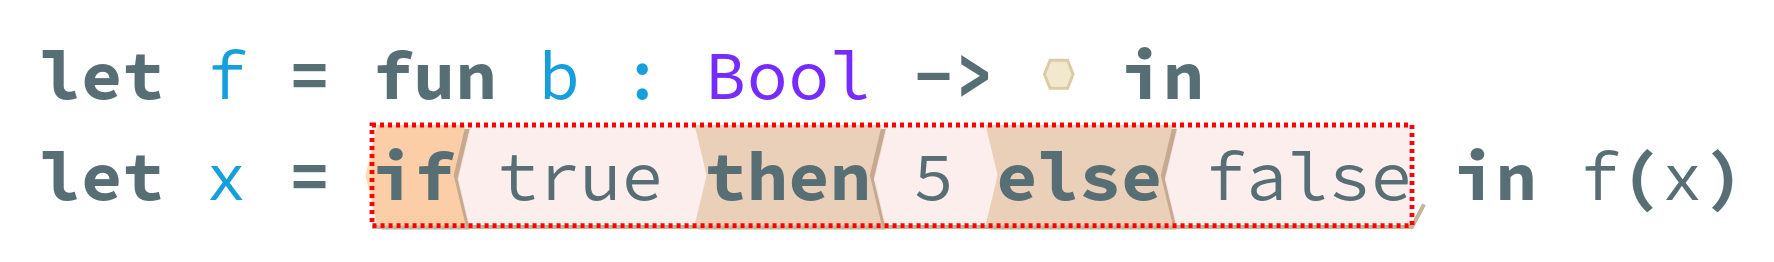
\includegraphics[width=0.9\linewidth]{media/inconsistent.png}
      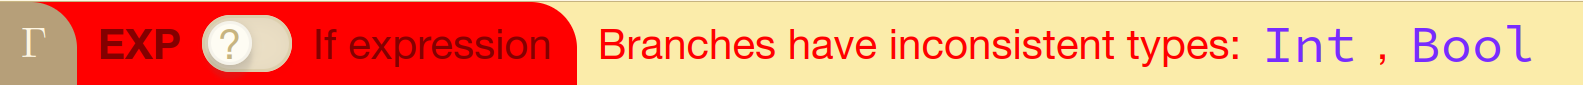
\includegraphics[width=0.9\linewidth]{media/inconsistent-ci.png}
    \end{center}
  }

  \note[item]<1-3>{Let's look for example at this program, in which we've a function f that takes a
    boolean---and does something}
  \note[item]<1-3>{x is determined by a conditional}
  \note[item]<1-3>{and f is applied to x}
  \note[item]<1-3>{We can immediately see that the branches of the conditional are mismatched wrt to
    typing, so there should be some sort of error diagnostic}
  \note[item]<4->{and in fact if we throw this at the OCaml compiler, it says, yes, there is, and it's
    on the false, having prioritized the first branch's integer}
  \note[item]<4->{ocamlc will stop here, but merlin, which powers editor services nowadays, will also
    say that there's another error on the usage of x, since it's determined x to be an int but f takes
    a bool}
  \note[item]<4->{OK, that's all well and good, so what about Haskell?}
  \note[item]<4->{Somewhat unexpectedly, it localizes the error to 5, complaining that it isn't an
    instance of Num Bool---this is presumably because of how type inference works for the Num type
    class}
  \note[item]<4->{Rust is a little different in that it prioritizes the first branch like OCaml but
    also suggests that the 5 is to blame}
  \note[item]<4->{Hazel, the programming environment our group is building, is still different,
    assigning the error to the entire conditional with the cursor inspector stating that the
    branches are inconsistent}
\end{frame}

\begin{frame}{Observations in practice}
  Today's tooling is error-resilient to a certain degree\pause, but \\[1em]

  \pause
  \begin{itemize}
    \item localization can be varied\pause, often guessing about \emph{user intent}

      \pause
    \item recovery necessitates reasoning without complete knowledge about types

      \pause
    \item decisions can influence other downstream decisions
  \end{itemize}

  \note[item]{Now obviously these languages all have different kinds of type systems, but from this
    informal exercise we can observe that practical systems are type error-resilient to a
    certain degree, but}
  \note[item]{decisions about how to localize can vary, and often tools will try to guess users'
    intentions about where to localize errors to}
  \note[item]{Then, to recover, they have to somehow operate with incomplete knowledge about the
    types at play}
  \note[item]{and together, upstream error localization decisions, once recovered from, can
    influence downstream decisions, sometimes unexpectedly}
  \note[item]{We think, therefore, that this subject would benefit greatly from rigorous treatment}
  \note[item]{Unfortunately, our current developments in theory don't reflect this reality}
\end{frame}

\begin{frame}{A definitional gap problem}
  \begin{center}
    Most of the code we write is \emph{ill-typed}\pause,
    but conventional language definitions
    \emph{only specify the meaning of well-typed programs}. \\[0.5em]

    \pause
    $\Gamma \vdash e : \tau$
  \end{center}
  \pause
  \[%
    \bm{\Downarrow}
  \]%

  \begin{center}
    If a type error appears \textcolor{RedOrange}{\textbf{anywhere}},\\
    the program is meaningless \textcolor{Red}{\textbf{everywhere}}.
  \end{center}

  \note[item]{Most of the code we write is ill-typed, but conventional language definitions are only
    concerned with the semantics of well-typed programs}
  \note[item]{This is made most obvious by the fact that our type systems look generally like some
    variation of this judgment form}
  \note[item]{So if a type error appears anywhere}
  \note[item]{as far as the specification are concerned, the program becomes meaningless as a whole}
\end{frame}

\begin{frame}{The goal}
  We'd like a way to formally specify type checkers that are capable of localizing and recovering
  from errors \\[1em]

  \pause
  \begin{emphbox}{Totality}
    These semantics should give meaning to \emph{all well-typed and ill-typed programs}.
  \end{emphbox}

  \note[item]{We'd like a way to alleviate this, by being able to create precise specifications for
    the typing semantics of these ill-typed programs, localizing and recovering from type errors along
    the way}
  \note[item]{And these type checker semantics should describe both well-typed and ill-typed
    programs}
  \note[item]{This notion we'll call totality, and it'll serve as a sort of guiding principle}
\end{frame}

\begin{frame}{This paper is about\ldots}
  \pause
  Uniting \emph{local} and \emph{global} type inference for principled total type error localization and
  recovery: \\[1em]

  \begin{itemize}
    \item<3-> the \textbf{marked lambda calculus}%
      \uncover<4->{%
        : a judgmental framework for bidirectional type error localization and recovery%
      }

    \item<5-> \textbf{type hole inference}%
      \uncover<6->{%
        : a global, constraint-based system \\
        that is neutral in error localization and recovery
      }
  \end{itemize}

  \only<1-4>{
  \note[item]{In this work, we've developed techniques to achieve total type error localization and
    recovery by elegantly blending local and global type inference}
  \note[item]{For the former, we present in tutorial-style the marked lambda calculus, a judgmental
    framework for type error localization and recovery for bidirectional type systems}
  \note[item]{We choose bidirectional systems as our starting point because it creates a flow of
    typing data that is conducive to intuitive error localization}
  }
  \only<5->{
  \note[item]{Then, we'll describe type hole inference, or how to layer a global constraint-based
    inference system atop the marked lambda calculus in a way that allows us to neatly combine the
    bidirectional and unification approaches for even better localization}
  \note[item]{While these two paradigms have been often thought of as opposing or alternative
    techniques, in this talk we'll hopefully see how they supplement each other}
  \note[item]{And hopefully you'll be able to see how these techniques are fairly generally and
    applicable}
  }
\end{frame}

\newcommand{\entails}{\ensuremath{\goodcolor{\colorOkSideJudge}{\vdash}}}
\newcommand{\syn}{\ensuremath{\goodcolor{\colorOkSideJudge}{\Rightarrow}}}
\newcommand{\ana}{\ensuremath{\goodcolor{\colorOkSideJudge}{\Leftarrow}}}

\newcommand{\ctxSyn}[3]{\ensuremath{#1 \entails #2 \syn #3}}
\newcommand{\ctxAna}[3]{\ensuremath{#1 \entails #2 \ana #3}}

\begin{frame}[fragile]{Marked lambda calculus: a tutorial}
  \textbf{Start:} a small gradually typed lambda calculus*
  %
  \[\begin{array}{rcl}
    \TMV  & \Coloneqq & \TUnknown \mid \TNum \mid \TBool \mid \TArrow{\TMV}{\TMV} \\
    \EMV  & \Coloneqq & x \mid \ELam{x}{\TMV}{\EMV} \mid \EAp{\EMV}{\EMV}
    \mid                   \ENumMV \mid \ETrue \mid \EFalse \mid \EIf{\EMV}{\EMV}{\EMV}
  \end{array}\]

  \pause

  \hphantom{\textbf{Start:} }with a standard bidirectional type system
  %
  \pause
  \[\begin{array}{rl}
    \ctxSyn{\ctx}{\EMV}{\TMV} & \text{\small ($\EMV$ synthesizes type $\TMV$)} \\
    \ctxAna{\ctx}{\EMV}{\TMV} & \text{\small ($\EMV$ analyzes against type $\TMV$)}
  \end{array}\]
  \pause
  *We need only the \emph{static semantics} for ill-typed programs!

  \note[item]{For the purposes of this short tutorial, we'll start with a small gradually typed lambda
    calculus}
  \note[item]{with a standard bidirectional type system}
  \note[item]{Now, we have here the unknown type, but in fact it's necessary as we'll see for
    ill-typed programs only, and we require then only the static semantics of the gradually typed
    lambda calculus}
\end{frame}

\begin{frame}[fragile]{Typing variable occurrences}
  Synthesizing the type of a variable is standard:
  \[%
    \inferrule[SVar]{
      \uncover<2->{\colorbox{highlight}{\inCtx{\ctx}{x}{\TMV}}}
    }{
      \ctxSyn{\ctx}{x}{\TMV}
    }
  \]%

  \uncover<3->{
    But what if $\notInCtx{\ctx}{x}$?
  }

  \note[item]{In our standard bidirectional type system, we would probably have a rule that looks
    like this incomplete one for synthesizing the type of a variable occurrence}
  \note[item]{We can conclude, of course, that x synthesizes tau if we have the pair in the context}
  \note[item]{OK, that's all well and good, but what if x isn't in scope?}
\end{frame}

\begin{frame}[fragile]
  How do we handle this failure case?

  \begin{lstlisting}[style=OCaml, escapechar=@]
let rec syn ctx e =
  match e with
    Var x ->
      match Ctx.lookup ctx x with
        Some ty -> @\only<1-3>{ty}\only<4>{\goodcolor{PineGreen}{Ok(ty)}}@
        None    -> @\goodcolor{red}{\only<1>{???}\only<2>{assert false}\only<3>{failwith (x ++ " is unbound")}\only<4>{Error(UnboundError(...))}}@
    ...
  \end{lstlisting}

  \only<1>{\phantom{Option 1}}
  \only<2>{Option 1: don't be ridiculous, that's impossible}
  \only<3>{Option 2: uh oh, not my problem}
  \only<4>{Option 3: uh oh, not my problem but explicitly}

  \note[item]{This failure case poses a problem if we were to try implementing this rule}
  \note[item]{An implementation of type synthesis in OCaml might look something like this code}
  \note[item]{where we thread a typing context and lookup variable occurrences}
  \note[item]{The None case corresponds exactly to being unable to satisfy the premise, and it's not
    immediately obvious what we should do}
  \note[item]{We could crash, though I don't think anyone would be very happy about this}
  \note[item]{More realistically, we might throw an exception with a diagnostic and leave it to the
    caller to handle}
  \note[item]{or similarly by returning an error value}
  \note[item]{In either case, we've aborted the type-checking early at the first error, and this
    just isn't going to cut it}
\end{frame}

\begin{frame}[fragile]
  We've \emph{localized} the error: \pause ``this occurrence of $x$ is unbound!'' \\[1em]

  \pause
  How can we \emph{recover}? \\[1em]

  \pause
  \textbf{Solution.} $\TUnknown$ \pause \hspace{1em} $\leftarrow$ unknown type

  \note[item]{At this point, we've localized the error successfully}
  \note[item]{But how can we recover?}
  \note[item]{You've probably guessed it by now, but we'll do so via the unknown type}
\end{frame}

\begin{frame}[fragile]{From type checking to marking}
  \textbf{Idea.} Augment the type checking process with \emph{marking}! \\[1em]

  \pause
  \begin{itemize}
    \item localize and report the error as a \emph{mark}
      \pause
      \begin{itemize}
        \item compiler messages

          \pause
        \item editor decorations
      \end{itemize}

      \pause
    \item use the unknown type to encapsulate missing type information
  \end{itemize}

  \note[item]{The idea is to augment the type checking process with marking}
  \note[item]{where we localize and report errors by adding marks}
  \note[item]{which intuitively correspond to compiler diagnostics or editor decorations}
  \note[item]{Then, we'll use the unknown type, which provides exactly the right mechanisms via
    the consistency relation to recover in a principled manner}
\end{frame}

\begin{frame}[fragile]{A two-layer calculus}
  Supplement the \emph{unmarked} surface syntax

  \[\begin{array}{rcl}
    \TMV  & \Coloneqq & \TUnknown \mid \TNum \mid \TBool \mid \TArrow{\TMV}{\TMV} \\
    \EMV  & \Coloneqq & x \mid \ELam{x}{\TMV}{\EMV} \mid \EAp{\EMV}{\EMV}
            \mid           \ENumMV \mid \ETrue \mid \EFalse
            \hphantom{\ \mid           \ECFree{x}} \\
  \end{array}\]

  \pause
  into a \emph{marked} one that contains \emph{error marks}:
  \[\begin{array}{rcl}
    \ECMV & \Coloneqq & x \mid \ECLam{x}{\TMV}{\ECMV} \mid \ECAp{\ECMV}{\ECMV}
            \mid           \ECNumMV \mid \ECTrue \mid \ECFalse
            \mid           \ECFree{x}
  \end{array}\]

  \pause
  $\ECFree{x}$ is a \emph{marked term} denoting a free occurrence of $x$

  \note[item]{We'll take the original syntax, which we call unmarked, and add the aforementioned
    error marks}
  \note[item]{For now, we've only a single error mark that denotes exactly the variable is free}
  \note[item]{In this talk and paper, all the error marks are given by fancy parentheses and a
    subscript in red, but it's important to remember that these are only symbolic representations of
    actual error diagnostics!}
  \note[item]{The box subscript here corresponds to the error of a free variable}
\end{frame}

\begin{frame}[fragile]
  Extend the original typing judgments
  \[\begin{array}{rl}
    \ctxSyn{\ctx}{\EMV}{\TMV} & \text{\small ($\EMV$ synthesizes type $\TMV$)} \\
    \ctxAna{\ctx}{\EMV}{\TMV} & \text{\small ($\EMV$ analyzes against type $\TMV$)}
  \end{array}\]

  \pause
  into the bidirectional \textbf{marking judgments}:
  \pause
  \[\begin{array}{rl}
    \ctxSynFixedInto{\ctx}{\EMV}{\ECMV}{\TMV} & \text{{\small ($\EMV$ is marked into $\ECMV$ and synthesizes type $\TMV$)}} \\ \pause
    \ctxAnaFixedInto{\ctx}{\EMV}{\ECMV}{\TMV} & \text{{\small ($\EMV$ is marked into $\ECMV$ and analyzes against type $\TMV$)}}
  \end{array}\]

  \note[item]{Now, we'll extend the original typing judgments into marking judgments}
  \note[item]{where unmarked expressions are marked into marked expressions}
  \note[item]{These now are the judgments that express the error-localizing and recovering type-checking process}
\end{frame}

\begin{frame}[fragile]{Marking free variables}
  One typing rule for variables 
  \[%
    \inferrule[SVar]{
      \inCtx{\ctx}{x}{\TMV}
    }{
      \ctxSyn{\ctx}{x}{\TMV}
    }
  \]%

  becomes two synthetic marking rules: 
  \begin{mathpar}
    \uncover<2->{
      \inferrule[MKSVar]{
        \inCtx{\ctx}{x}{\TMV}
      }{
        \ctxSynFixedInto{\ctx}{x}{x}{\TMV}
      }
    }

    \uncover<3->{
      \inferrule[MKSFree]{
        \notInCtx{\ctx}{x}
      }{
        \uncover<3->{\ctxSynFixedInto{\ctx}{x}{\uncover<4->{\ECFree{x}}}{\uncover<5->{\TUnknown}}}
      }
    }
  \end{mathpar}

  \note[item]{It's hopefully straightforward to see how we can determine the rules for the marking
    judgments}
  \note[item]{Thinking about both the success and failure cases, our synthetic typing rule for
    variables becomes two synthetic marking rules}
  \note[item]{In the success case we don't need to mark any errors}
  \note[item]{And in the failure case we'll mark x with the free variable mark and synthesize the
    unknown type}
\end{frame}

\begin{frame}[fragile]{A total marking}
  \begin{emphbox}{Guiding principle (totality)}
    These typing semantics should describe \\
    \emph{all syntactically well-formed programs}.
  \end{emphbox}
  %
  \pause
  \begin{center}
    $\bm{\Downarrow}$
  \end{center}

  \begin{emphbox}{Theorem 2.1. Marking Totality}
    \pause
    For all $\ctx$ and $\EMV$,
      $\exists \ECMV, \TMV$
        s.t. $\ctxSynFixedInto{\ctx}{\EMV}{\ECMV}{\TMV}$. \\
    For all $\ctx$, $\EMV$, and $\TMV$,
      $\exists \ECMV$
        s.t. $\ctxAnaFixedInto{\ctx}{\EMV}{\ECMV}{\TMV}$.
  \end{emphbox}
\end{frame}

\begin{frame}[fragile]{Marking function application}
  \textbf{Example.} The synthetic typing rule for function application:
  %
  \begin{mathpar}
    \inferrule[SAp]{
      \ctxSyn{\ctx}{\EMV_1}{\TMV} \\
      \matchedArrow{\TMV}{\TMV_1}{\TMV_2} \\
      \ctxAna{\ctx}{\EMV_2}{\TMV_1}
    }{
      \ctxSyn{\ctx}{\EAp{\EMV_1}{\EMV_2}}{\TMV_2}
    } \\

    \inferrule[TMAUnknown]{ }{
      \matchedArrow{\TUnknown}{\TUnknown}{\TUnknown}
    }

    \inferrule[TMAArr]{ }{
      \matchedArrow{\TArrow{\TMV_1}{\TMV_2}}{\TMV_1}{\TMV_2}
    }
  \end{mathpar}
\end{frame}

\begin{frame}[fragile]
  \ldots\ becomes the synthetic marking rule:
  \[%  
    \uncover<2->{
      \inferrule[MKSAp]{
      \uncover<3->{\ctxSynFixedInto{\ctx}{\EMV_1}{\ECMV_1}{\TMV}} \\
      \uncover<4->{\matchedArrow{\TMV}{\TMV_1}{\TMV_2}} \\
      \uncover<5->{\ctxAnaFixedInto{\ctx}{\EMV_2}{\ECMV_2}{\TMV_1}} \\
    }{
      \ctxSynFixedInto{\ctx}{\EAp{\EMV_1}{\EMV_2}}{\uncover<6->{\ECAp{\ECMV_1}{\ECMV_2}}}{\uncover<7->{\TMV_2}}
    }
    }
  \]%

  \uncover<8->{
    But what if $\TMV$ doesn't match an arrow type, $\notMatchedArrow{\TMV}$, \\
    \ie, $\EMV_1$ can't be applied as a function, \eg, in $\EAp{\ENum{5}}{\ETrue}$?
  }
\end{frame}

\begin{frame}[fragile]
  Introduce the mark $\ECApSynNonMatchedArrow{\ECMV_1}{\ECMV_2}$ for this error:
  \[%
    \ECMV \Coloneqq \cdots \mid \ECFree{x} \mid \only<1->{\ECApSynNonMatchedArrow{\ECMV}{\ECMV}}
  \]%
  \uncover<2->{
  \begin{mathpar}
    \inferrule[MKSAp1]{
      \ctxSynFixedInto{\ctx}{\EMV_1}{\ECMV_1}{\TMV} \\
      \matchedArrow{\TMV}{\TMV_1}{\TMV_2} \\
      \ctxAnaFixedInto{\ctx}{\EMV_2}{\ECMV_2}{\TMV_1} \\
    }{
      \ctxSynFixedInto{\ctx}{\EAp{\EMV_1}{\EMV_2}}{\ECAp{\ECMV_1}{\ECMV_2}}{\TMV_2}
    }

    \uncover<3->{
      \inferrule[MKSAp2]{
        \ctxSynFixedInto{\ctx}{\EMV_1}{\ECMV_1}{\TMV} \\
        \notMatchedArrow{\TMV} \\
        \uncover<4->{\ctxAnaFixedInto{\ctx}{\EMV_2}{\ECMV_2}{\TUnknown}}
      }{
        \ctxSynFixedInto{\ctx}{\EAp{\EMV_1}{\EMV_2}}{\uncover<5->{\ECApSynNonMatchedArrow{\ECMV_1}{\ECMV_2}}}{\uncover<6->{\TUnknown}}
      }
    }
  \end{mathpar}
  }
\end{frame}

\begin{frame}{The marked lambda calculus, altogether}
  \begin{center}
    \begin{tikzpicture}[box/.style={align=left, fill=white}]
      \Alt<4->{
        \node[box] (unmarked) {
          \begin{minipage}[t][1.5cm]{4cm}
            \emph{unmarked language} \\
            $\ctxSynTypeU{\ctx}{\EMV}{\TMV}$ \\
            $\ctxAnaTypeU{\ctx}{\EMV}{\TMV}$
          \end{minipage}
        };
      }{
        \node[box] (unmarked) {
          \begin{minipage}[t][1.5cm]{4cm}
            \emph{original language} \\
            $\ctxSyn{\ctx}{\EMV}{\TMV}$ \\
            $\ctxAna{\ctx}{\EMV}{\TMV}$
          \end{minipage}
        };
      }

      \node[box, visible on=<2->] (marking) [right=2.5cm of unmarked] {
        \begin{minipage}[t][1.5cm]{4cm}
          \emph{marking} \\
          $\ctxSynFixedInto{\ctx}{\EMV}{\ECMV}{\TMV}$ \\
          $\ctxAnaFixedInto{\ctx}{\EMV}{\ECMV}{\TMV}$
        \end{minipage}
      };

      \node[box, visible on=<3->] (marked) [below=2.5cm of marking] {
        \begin{minipage}[t][1.5cm]{4cm}
          \emph{marked language} \\
          $\ctxSynTypeM{\ctx}{\ECMV}{\TMV}$ \\
          $\ctxAnaTypeM{\ctx}{\ECMV}{\TMV}$
        \end{minipage}
      };

      \node[box, visible on=<5->] (erasure) [below=2.5cm of unmarked] {
        \begin{minipage}[t][1.5cm]{4cm}
          \emph{mark erasure} \\
          $\erase{\ECMV}$
        \end{minipage}
      };

      \draw[-latex, dashed, shorten >=5pt, visible on=<2->] (unmarked) -- (marking) node[midway, above] () {\small \emph{derive}};
      \draw[-latex, shorten >=5pt, visible on=<3->] (unmarked) to[bend left=20] (marked);
      \draw[-latex, shorten <=5pt, visible on=<5->] (marked)   to[bend left=20] (unmarked);
    \end{tikzpicture}
  \end{center}
\end{frame}

\begin{frame}[fragile]
  \begin{emphbox}{Theorem 2.2. Marking Well-Formedness}
    If $\ctxSynFixedInto{\ctx}{\EMV}{\ECMV}{\TMV}$,
      then $\ctxSynTypeM{\ctx}{\ECMV}{\TMV}$
        and $\erasesTo{\ECMV}{\EMV}$. \\
    If $\ctxAnaFixedInto{\ctx}{\EMV}{\ECMV}{\TMV}$,
      then $\ctxAnaTypeM{\ctx}{\ECMV}{\TMV}$
        and $\erasesTo{\ECMV}{\EMV}$.
  \end{emphbox}

  \pause
  \begin{emphbox}{Theorem 2.3(1). Marking Well-Typed Terms}
    If $\ctxSynTypeU{\ctx}{\EMV}{\TMV}$,
      then $\exists \ECMV$
        s.t. $\ctxSynFixedInto{\ctx}{\EMV}{\ECMV}{\TMV}$
        and $\markless{\ECMV}$. \\
    If $\ctxAnaTypeU{\ctx}{\EMV}{\TMV}$,
      then $\exists \ECMV$
        s.t. $\ctxAnaFixedInto{\ctx}{\EMV}{\ECMV}{\TMV}$
        and $\markless{\ECMV}$.
  \end{emphbox}
\end{frame}

\begin{frame}[fragile]{The recipe}
  \begin{itemize}
    \item Begin with a bidirectional gradually typed language

      \pause
    \item Derive marking rules from each typing rule
      %
      \begin{itemize}
        \item Consider the ``success'' case
        \item Consider the ``failure'' cases, introducing error marks
      \end{itemize}

      \pause
    \item \emph{Not} prescriptive \wrt{} localization strategy,\pause \eg,
      %
      \begin{itemize}
        \item use different marks, localize somewhere else, etc.
          \pause
        \item extend the judgments to accumulate facts that inform localization decisions
      \end{itemize}
  \end{itemize}
\end{frame}

\begin{frame}[fragile]{Marking local inconsistencies}
  The standard subsumption principle:
  \[%
    \inferrule[UASubsume]{
      \ctxSynTypeU{\ctx}{\EMV}{\TMV'} \\
      \consistent{\TMV}{\TMV'}
    }{
      \ctxAnaTypeU{\ctx}{\EMV}{\TMV}
    }
  \]%

  \pause
  becomes the analytic marking and (marked) typing rules:
  %
  \begin{mathpar}
    \inferrule[MKASubsume]{
      \ctxSynFixedInto{\ctx}{\EMV}{\ECMV}{\TMV'} \\
      \consistent{\TMV}{\TMV'}
    }{
      \ctxAnaFixedInto{\ctx}{\EMV}{\ECMV}{\TMV}
    }

    % \inferrule[MASubsume]{
      % \ctxSynTypeM{\ctx}{\ECMV}{\TMV'} \\
      % \consistent{\TMV}{\TMV'}
    % }{
      % \ctxAnaTypeM{\ctx}{\ECMV}{\TMV}
    % }
  \end{mathpar}
\end{frame}

\begin{frame}
  What if $\inconsistent{\TMV}{\TMV'}$, \eg, in $\ELam{f}{\TArrow{\TNum}{\TNum}}{\EAp{f}{\goodcolor{Red}{\ETrue}}}$?

  \pause
  \[%
    \ECMV \Coloneqq \cdots \mid \ECFree{x} \mid \ECApSynNonMatchedArrow{\ECMV}{\ECMV} \mid \colorbox{highlight}{\ECInconType{\ECMV}}
  \]%

  \pause
  \begin{mathpar}
    \inferrule[MKASubsume]{
      \ctxSynFixedInto{\ctx}{\EMV}{\ECMV}{\TMV'} \\
      \consistent{\TMV}{\TMV'}
    }{
      \ctxAnaFixedInto{\ctx}{\EMV}{\ECMV}{\TMV}
    }

    \inferrule[MKAInconsistentTypes]{
      \ctxSynFixedInto{\ctx}{\EMV}{\ECMV}{\TMV'} \\
      \inconsistent{\TMV}{\TMV'}
    }{
      \ctxAnaFixedInto{\ctx}{\EMV}{\ECInconType{\ECMV}}{\TMV}
    }

    % \inferrule[MAInconsistentTypes]{
      % \ctxSynTypeM{\ctx}{\ECMV}{\TMV'} \\
      % \inconsistent{\TMV}{\TMV'}
    % }{
      % \ctxAnaTypeM{\ctx}{\ECInconType{\ECMV}}{\TMV}
    % }
  \end{mathpar}
\end{frame}

\begin{frame}{Marking \underline{global} inconsistencies}
  Consider this program:
  \[%
    \ELam{f}{\TUnknown}{\EAp{f}{(\EPlus{f}{1})}}
  \]%

  \pause
  $f : \TUnknown$, so the bidirectional system operates gradually, \pause
  but $f$ is 
  %
  \pause
  \begin{enumerate}
    \item applied as a function \pause (a function?)
      \pause
    \item an operand of $+$ \pause (a number?)
  \end{enumerate}

  \pause
  \vspace{1em}
  \emph{Constraint-based type checking would have caught this!}
\end{frame}

\begin{frame}{Layers on layers}
  Get the best of both worlds by layering \textbf{constraint-based inference} 
  atop the marked lambda calculus

  \vspace{1em}
  \pause
  \begin{itemize}
    \item 
  \end{itemize}
\end{frame}

\begin{frame}{Bidirectional and unification, together}
  The two systems supplement each other: \\[1em]

  \pause
  \begin{itemize}
    \item \emph{marked lambda calculus}: \\
      a general recipe for local type error localization and recovery

      \pause
    \item \emph{type hole inference}: \\
      a workflow for handling globally inconsistent constraints
  \end{itemize}

  \vspace{1em}
  \pause
  Consider using these techniques for your next language!
\end{frame}

\begin{frame}{More in the paper and artifact}
  \begin{itemize}
    \item A full description of the marked lambda calculus\pause, and

      \begin{itemize}
        \item full metatheory\pause, also mechanized
          \textcolor{MidnightBlue}{[\href{https://github.com/hazelgrove/error-localization-agda}{hazelgrove/error-localization-agda}]}

          \pause
        \item extensions to richer typing features \\ \pause
          (parametric polymorphism and destructuring let)

          \pause
        \item connections to structured editing
      \end{itemize}

      \pause
    \item A more thorough discussion of type hole inference\pause, and

      \begin{itemize}
        \item filling expression holes

          \pause
        \item polymorphic generalization
      \end{itemize}

      \pause
    \item Implementations of both in Hazel
      \textcolor{BrickRed}{\small[\href{https://hazel.org}{hazel.org}]}
      \textcolor{MidnightBlue}{\small[\href{https://github.com/hazelgrove/hazel}{hazelgrove/hazel}]}
  \end{itemize}
\end{frame}


\end{document}
